\documentclass[../main]{subfiles}

\questiontrue
\solutiontrue

\begin{document}
    \ifquestion
    
	\section{Plutonian Atmosphere II}

The scientist José Lagranja, a resident of the planet Pluto II, in his planetary studies of his home planet, aimed to develop a model for the planet’s atmosphere. He observed that the gases composing the atmosphere behave as ideal gases.

The planet Pluto II has radius $R$, mass $M$, and an atmosphere composed of particles of mass $m$.

\parte{A}{Physical Modeling}

\ut{A.1} Given that the atmosphere is in thermal equilibrium, that the temperature at its surface is $T(R)$, and that the radial derivative of temperature at its surface is $\dot{T}(R)$, find an expression for the temperature of the atmosphere at a distance $r$ from the planet's center.

\ut{A.2} Using the equations of hydrodynamic equilibrium and the ideal gas law, show an expression for the density of the gases at a distance $r$ from the planet’s center. Express your answer in terms of $\rho(R)$, the density of the atmosphere at the planet’s surface.

\ut{A.3} Finally, find an expression for the pressure of the atmosphere at a distance $r$ from the planet’s center.

\ut{A.4} Consider that the atmosphere of Pluto II consists of a very thin layer (compared to the planet’s radius $R$) of thickness $e$, and that, coincidentally, the temperature at the planet’s surface is given by: $T(R) = \dfrac{GM m E}{k R^2}$. Determine a simplified expression with the detailed approximations for $T(r)$ and for $\rho(r)$.

\parte{B}{Atmospheric Distortion}

\ut{B.1} Consider a light ray arriving at the atmosphere with an angle $\theta$ relative to the normal of the outermost layer. Due to the variable refractive index of the different layers, the trajectory of the ray is distorted into a curve, as shown in Figure \ref{fig:binabina}:

	\begin{figure}[htpb]
	\centering
		
		
		\tikzset{every picture/.style={line width=0.75pt}} %set default line width to 0.75pt        
		
		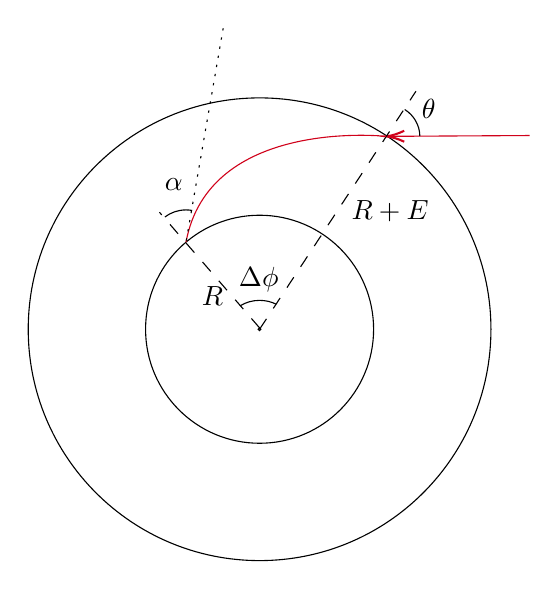
\begin{tikzpicture}[x=0.75pt,y=0.75pt,yscale=-0.8,xscale=0.8]
			%uncomment if require: \path (0,436); %set diagram left start at 0, and has height of 436
			
			%Shape: Circle [id:dp19485467879625507] 
			\draw   (85.5,187.17) .. controls (85.5,149.24) and (116.24,118.5) .. (154.17,118.5) .. controls (192.09,118.5) and (222.83,149.24) .. (222.83,187.17) .. controls (222.83,225.09) and (192.09,255.83) .. (154.17,255.83) .. controls (116.24,255.83) and (85.5,225.09) .. (85.5,187.17) -- cycle ;
			%Shape: Circle [id:dp13391993851810668] 
			\draw   (14.83,187.17) .. controls (14.83,110.21) and (77.21,47.83) .. (154.17,47.83) .. controls (231.12,47.83) and (293.5,110.21) .. (293.5,187.17) .. controls (293.5,264.12) and (231.12,326.5) .. (154.17,326.5) .. controls (77.21,326.5) and (14.83,264.12) .. (14.83,187.17) -- cycle ;
			%Straight Lines [id:da6574242355053763] 
			\draw [color={rgb, 255:red, 208; green, 2; blue, 27 }  ,draw opacity=1 ]   (316.8,70.5) -- (232.33,70.99) ;
			\draw [shift={(230.33,71)}, rotate = 359.67] [color={rgb, 255:red, 208; green, 2; blue, 27 }  ,draw opacity=1 ][line width=0.75]    (10.93,-3.29) .. controls (6.95,-1.4) and (3.31,-0.3) .. (0,0) .. controls (3.31,0.3) and (6.95,1.4) .. (10.93,3.29)   ;
			%Shape: Circle [id:dp7617608465256409] 
			\draw   (153.36,187.17) .. controls (153.36,186.72) and (153.72,186.36) .. (154.17,186.36) .. controls (154.61,186.36) and (154.97,186.72) .. (154.97,187.17) .. controls (154.97,187.61) and (154.61,187.97) .. (154.17,187.97) .. controls (153.72,187.97) and (153.36,187.61) .. (153.36,187.17) -- cycle ;
			%Straight Lines [id:da9055512085521675] 
			\draw  [dash pattern={on 4.5pt off 4.5pt}]  (154.17,187.17) -- (248.33,43.83) ;
			%Shape: Arc [id:dp7167637284723158] 
			\draw  [draw opacity=0] (241.57,54.81) .. controls (247.01,58.27) and (250.61,64.16) .. (250.67,70.85) -- (230.33,71) -- cycle ; \draw   (241.57,54.81) .. controls (247.01,58.27) and (250.61,64.16) .. (250.67,70.85) ;
			%Curve Lines [id:da16809361305465553] 
			\draw [color={rgb, 255:red, 208; green, 2; blue, 27 }  ,draw opacity=1 ]   (109.86,134.71) .. controls (123.5,60.63) and (227,70.63) .. (230.33,71) ;
			%Straight Lines [id:da37934178134811636] 
			\draw  [dash pattern={on 4.5pt off 4.5pt}]  (154.17,186.36) -- (93.86,116.71) ;
			%Shape: Arc [id:dp9767984317707079] 
			\draw  [draw opacity=0] (142.36,173.11) .. controls (145.69,171.01) and (149.77,169.77) .. (154.17,169.77) .. controls (157.8,169.77) and (161.21,170.61) .. (164.16,172.09) -- (154.17,187.77) -- cycle ; \draw   (142.36,173.11) .. controls (145.69,171.01) and (149.77,169.77) .. (154.17,169.77) .. controls (157.8,169.77) and (161.21,170.61) .. (164.16,172.09) ;
			%Straight Lines [id:da4841974246097642] 
			\draw  [dash pattern={on 0.84pt off 2.51pt}]  (132.25,5.88) -- (109.86,134.71) ;
			%Shape: Arc [id:dp10348939914575994] 
			\draw  [draw opacity=0] (97.14,119.56) .. controls (100.62,116.89) and (105.04,115.3) .. (109.86,115.3) .. controls (111.13,115.3) and (112.38,115.41) .. (113.59,115.62) -- (109.86,134.71) -- cycle ; \draw   (97.14,119.56) .. controls (100.62,116.89) and (105.04,115.3) .. (109.86,115.3) .. controls (111.13,115.3) and (112.38,115.41) .. (113.59,115.62) ;
			
			% Text Node
			\draw (250.33,47.23) node [anchor=north west][inner sep=0.75pt]    {$\theta $};
			% Text Node
			\draw (208,107.89) node [anchor=north west][inner sep=0.75pt]    {$R+E$};
			% Text Node
			\draw (117.81,159.89) node [anchor=north west][inner sep=0.75pt]    {$R$};
			% Text Node
			\draw (140.15,148.2) node [anchor=north west][inner sep=0.75pt]    {$\Delta \phi $};
			% Text Node
			\draw (95.5,94.7) node [anchor=north west][inner sep=0.75pt]    {$\alpha $};
			
			
		\end{tikzpicture}

\caption{Demonstration of the refraction caused by the planet’s atmosphere for a ray with an incidence angle $\theta$}
\label{fig:binabina}

\end{figure}

Note that, in the end, the celestial object in question is observed at a zenith distance $\alpha$. Find $\alpha$ knowing that the refractive index at a distance $r$ from the planet’s center is given by: $n(r)=n_0 r^{-1}$ for $R \le r \le R+E$, such that at the outer edge of the atmosphere this index equals that of vacuum.

\ut{B.2} Using the specified approximations, find $\Delta \phi$.

\ut{B.3} Knowing that the opacity of the atmospheric gases is constant and equal to $\kappa$, find the change in magnitude $\Delta m$ caused by atmospheric absorption for an object at zenith angle $z$.

\ut{B.4} Lagranja also studied two stars: AMX-13 and TUC-33. He knows that the parallax of these stars, disregarding atmospheric effects, is $p_a = 0.13''$ and $p_t = 0.33''$, respectively. Knowing that, at a given moment of his observation, Lagranja notes that the zenith distance of AMX-13 is $25^\circ$ and that of TUC-33 is $46^\circ$, that the azimuthal separation between them is $36^\circ$, and that the ratio $\dfrac{E}{R} = 3.3 \cdot 10^{-2}$. Find the distance between the stars in parsecs.

\clearpage

\fi

\ifsolution

\section{Plutonian Atmosphere II}

\parte{A}{Physical Modeling}

\ut{A.1} First, separate the atmosphere into infinitesimal layers of thickness $dr$. Each of these layers has a slightly different temperature from its neighbors, which causes heat to be transferred primarily through conduction.

Consider the following layer $dr$ of the atmosphere, located at a distance $r$ from the center:

\begin{figure}[htpb]
	\centering
		
		
		\tikzset{every picture/.style={line width=0.75pt}} %set default line width to 0.75pt        
		
		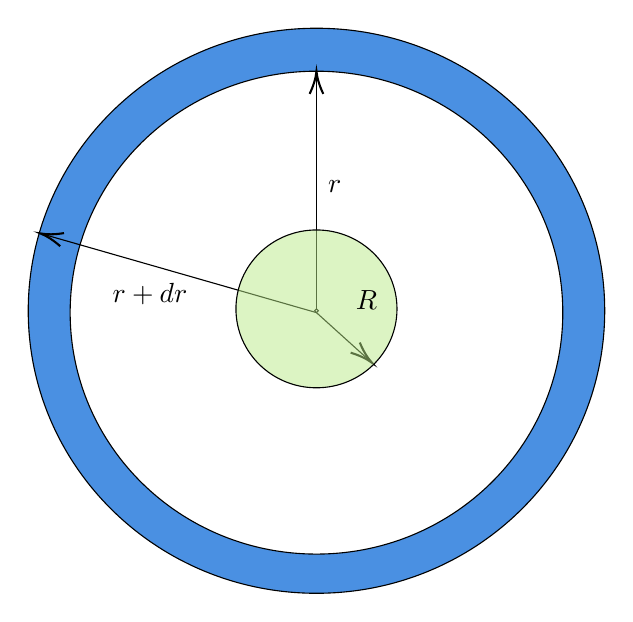
\begin{tikzpicture}[x=0.75pt,y=0.75pt,yscale=-1,xscale=1]
			%uncomment if require: \path (0,436); %set diagram left start at 0, and has height of 436
			
			%Shape: Ellipse [id:dp6074509730747526] 
			\draw  [color={rgb, 255:red, 0; green, 0; blue, 0 }  ,draw opacity=1 ] (166.86,285.27) .. controls (166.86,264.27) and (184.23,247.25) .. (205.66,247.25) .. controls (227.08,247.25) and (244.45,264.27) .. (244.45,285.27) .. controls (244.45,306.27) and (227.08,323.3) .. (205.66,323.3) .. controls (184.23,323.3) and (166.86,306.27) .. (166.86,285.27) -- cycle ;
			%Shape: Ellipse [id:dp5735691548943638] 
			\draw  [color={rgb, 255:red, 0; green, 0; blue, 0 }  ,draw opacity=1 ][fill={rgb, 255:red, 74; green, 144; blue, 226 }  ,fill opacity=1 ] (62.25,283.38) .. controls (62.25,208.2) and (124.43,147.26) .. (201.12,147.26) .. controls (277.82,147.26) and (340,208.2) .. (340,283.38) .. controls (340,358.56) and (277.82,419.5) .. (201.12,419.5) .. controls (124.43,419.5) and (62.25,358.56) .. (62.25,283.38) -- cycle ;
			%Shape: Ellipse [id:dp8039787945646049] 
			\draw  [color={rgb, 255:red, 0; green, 0; blue, 0 }  ,draw opacity=1 ][fill={rgb, 255:red, 255; green, 255; blue, 255 }  ,fill opacity=1 ] (82.45,284.28) .. controls (82.45,220.04) and (135.58,167.96) .. (201.12,167.96) .. controls (266.67,167.96) and (319.8,220.04) .. (319.8,284.28) .. controls (319.8,348.53) and (266.67,400.61) .. (201.12,400.61) .. controls (135.58,400.61) and (82.45,348.53) .. (82.45,284.28) -- cycle ;
			%Straight Lines [id:da12694003646616947] 
			\draw    (201.12,282.47) -- (201.12,169.96) ;
			\draw [shift={(201.12,167.96)}, rotate = 90] [color={rgb, 255:red, 0; green, 0; blue, 0 }  ][line width=0.75]    (10.93,-3.29) .. controls (6.95,-1.4) and (3.31,-0.3) .. (0,0) .. controls (3.31,0.3) and (6.95,1.4) .. (10.93,3.29)   ;
			%Shape: Ellipse [id:dp07070676644738616] 
			\draw   (200.2,283.38) .. controls (200.2,282.88) and (200.61,282.47) .. (201.12,282.47) .. controls (201.64,282.47) and (202.05,282.88) .. (202.05,283.38) .. controls (202.05,283.88) and (201.64,284.28) .. (201.12,284.28) .. controls (200.61,284.28) and (200.2,283.88) .. (200.2,283.38) -- cycle ;
			%Straight Lines [id:da5458168924144797] 
			\draw    (201.12,284.28) -- (69.99,246.66) ;
			\draw [shift={(68.07,246.11)}, rotate = 16.01] [color={rgb, 255:red, 0; green, 0; blue, 0 }  ][line width=0.75]    (10.93,-3.29) .. controls (6.95,-1.4) and (3.31,-0.3) .. (0,0) .. controls (3.31,0.3) and (6.95,1.4) .. (10.93,3.29)   ;
			%Straight Lines [id:da8167468911094893] 
			\draw    (201.12,284.28) -- (226.41,307.13) ;
			\draw [shift={(227.9,308.47)}, rotate = 222.09] [color={rgb, 255:red, 0; green, 0; blue, 0 }  ][line width=0.75]    (10.93,-3.29) .. controls (6.95,-1.4) and (3.31,-0.3) .. (0,0) .. controls (3.31,0.3) and (6.95,1.4) .. (10.93,3.29)   ;
			%Shape: Ellipse [id:dp2572895401483444] 
			\draw  [fill={rgb, 255:red, 184; green, 233; blue, 134 }  ,fill opacity=0.49 ] (162.33,282.47) .. controls (162.33,261.47) and (179.7,244.45) .. (201.12,244.45) .. controls (222.55,244.45) and (239.92,261.47) .. (239.92,282.47) .. controls (239.92,303.47) and (222.55,320.49) .. (201.12,320.49) .. controls (179.7,320.49) and (162.33,303.47) .. (162.33,282.47) -- cycle ;
			
			% Text Node
			\draw (205.43,219.61) node [anchor=north west][inner sep=0.75pt]    {$r$};
			% Text Node
			\draw (101.64,268.79) node [anchor=north west][inner sep=0.75pt]    {$r+dr$};
			% Text Node
			\draw (218.81,272.45) node [anchor=north west][inner sep=0.75pt]    {$R$};
			
			
		\end{tikzpicture}
	
\caption{Two-dimensional representation of the Plutonian II atmosphere distribution}
\end{figure}

For thermal equilibrium to occur, it is necessary that the heat flux entering the layer at $r$ from the layer at $r-dr$ is equal to the heat flux leaving $r$ towards $r+dr$, as shown in the scheme below:

	\begin{figure}[htpb]
		\centering
		
		\tikzset{every picture/.style={line width=0.75pt}} %set default line width to 0.75pt        
		
		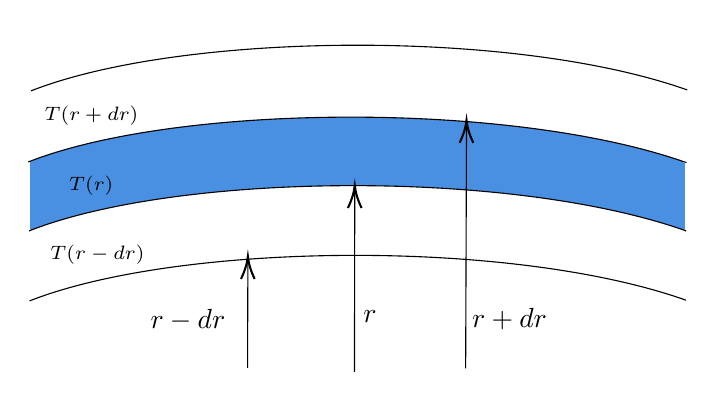
\begin{tikzpicture}[x=0.75pt,y=0.75pt,yscale=-1,xscale=1]
			%uncomment if require: \path (0,436); %set diagram left start at 0, and has height of 436
			
			%Curve Lines [id:da30787100119627997] 
			\draw [color={rgb, 255:red, 0; green, 0; blue, 0 }  ,draw opacity=1 ]   (34.67,167.76) .. controls (106.65,139.44) and (267.35,138.03) .. (351.03,167.75) ;
			%Curve Lines [id:da11127295832830786] 
			\draw    (34.79,201.53) .. controls (106.77,173.21) and (267.35,171.45) .. (351.03,201.17) ;
			%Curve Lines [id:da2795200461367824] 
			\draw [fill={rgb, 255:red, 74; green, 144; blue, 226 }  ,fill opacity=1 ]   (34.17,134.58) .. controls (106.15,106.26) and (267.65,105.19) .. (351.33,134.92) ;
			%Curve Lines [id:da49990360202475137] 
			\draw    (35.49,100.34) .. controls (107.47,72.02) and (267.98,70.15) .. (351.67,99.88) ;
			%Shape: Rectangle [id:dp6096088766137286] 
			\draw  [color={rgb, 255:red, 255; green, 255; blue, 255 }  ,draw opacity=0 ][fill={rgb, 255:red, 74; green, 144; blue, 226 }  ,fill opacity=1 ] (35.03,134.45) -- (350.38,134.45) -- (350.38,166.95) -- (35.03,166.95) -- cycle ;
			%Curve Lines [id:da19175358809778342] 
			\draw [fill={rgb, 255:red, 255; green, 255; blue, 255 }  ,fill opacity=1 ]   (34.67,167.76) .. controls (106.65,139.44) and (267.35,138.03) .. (351.03,167.75) ;
			%Straight Lines [id:da6628818912007384] 
			\draw    (139.84,233.82) -- (140,182.03) ;
			\draw [shift={(140,180.03)}, rotate = 90.18] [color={rgb, 255:red, 0; green, 0; blue, 0 }  ][line width=0.75]    (10.93,-3.29) .. controls (6.95,-1.4) and (3.31,-0.3) .. (0,0) .. controls (3.31,0.3) and (6.95,1.4) .. (10.93,3.29)   ;
			%Straight Lines [id:da8757149805483593] 
			\draw    (191.34,235.67) -- (191.5,147.82) ;
			\draw [shift={(191.5,145.82)}, rotate = 90.11] [color={rgb, 255:red, 0; green, 0; blue, 0 }  ][line width=0.75]    (10.93,-3.29) .. controls (6.95,-1.4) and (3.31,-0.3) .. (0,0) .. controls (3.31,0.3) and (6.95,1.4) .. (10.93,3.29)   ;
			%Straight Lines [id:da5331034047170613] 
			\draw    (244.92,233.98) -- (245.34,116.42) ;
			\draw [shift={(245.34,114.42)}, rotate = 90.2] [color={rgb, 255:red, 0; green, 0; blue, 0 }  ][line width=0.75]    (10.93,-3.29) .. controls (6.95,-1.4) and (3.31,-0.3) .. (0,0) .. controls (3.31,0.3) and (6.95,1.4) .. (10.93,3.29)   ;
			
			% Text Node
			\draw (91.84,204.45) node [anchor=north west][inner sep=0.75pt]  [font=\normalsize]  {$r-dr$};
			% Text Node
			\draw (246.82,203.95) node [anchor=north west][inner sep=0.75pt]  [font=\normalsize]  {$r+dr$};
			% Text Node
			\draw (194.38,204.88) node [anchor=north west][inner sep=0.75pt]  [font=\normalsize]  {$r$};
			% Text Node
			\draw (43.6,173.25) node [anchor=north west][inner sep=0.75pt]  [font=\scriptsize]  {$T( r-dr)$};
			% Text Node
			\draw (52.59,140.14) node [anchor=north west][inner sep=0.75pt]  [font=\scriptsize]  {$T( r)$};
			% Text Node
			\draw (40.8,106.5) node [anchor=north west][inner sep=0.75pt]  [font=\scriptsize]  {$T( r+dr)$};
			
			
		\end{tikzpicture}
	
\caption{Radial variation of temperature in the planet's atmosphere}
\end{figure}

The energy flux (power) transferred by conduction can be found using Fourier's law:

$$\phi=\frac{kA\Delta T}{L}$$

Adapting this to the conditions of the problem and setting the net flux in layer $r$ to zero:

$$\frac{k(4\pi r^2)(T(r-dr)-T(r))}{dr}-\frac{k(4\pi(r+dr)^2)(T(r)-T(r+dr))}{dr}=0$$

Note that we can divide both sides of the equation by $4\pi k$, and simplify $\dfrac{T(y+dy)-T(y)}{dy}=\dfrac{dT(y)}{dy}$:

$$r^2\frac{dT(r-dr)}{dr}=(r^2+2rdr)\frac{dT(r)}{dr}$$

Combining like terms (multiples of $r^2$), we have:

$$-2rdr\frac{dT(r)}{dr}=r^2\left(\frac{dT(r)}{dr}-\frac{dT(r-dr)}{dr} \right) $$

$$-2r\frac{dT(r)}{dr}=r^2\frac{\left(\frac{dT(r)}{dr}-\frac{dT(r-dr)}{dr} \right)}{dr}=r^2\frac{d^2T(r-dr)}{dr^2} $$

However, in the limit $dr\rightarrow0$: $\dfrac{d^2T(r-dr)}{dr^2}\rightarrow \dfrac{d^2T(r)}{dr^2}$. Using the notation provided in the problem statement (which indicates the derivative from points above the function):

$$-2r\dot{T}(r)=r^2\ddot{T}(r)\rightarrow \frac{d\dot{T}(r)}{\dot{T}(r)}=-2\frac{dr}{r}$$

$$\int_{\dot{T}(R)}^{\dot{T}(r)}\frac{d\dot{T}(r)}{\dot{T}(r)}=-2\int_R^r\frac{dr}{r}$$

$$\therefore \dot{T}(r)=\frac{dT(r)}{dr}=\dot{T}(R)\left(\frac{R}{r} \right)^2 $$

$$\int_{T(R)}^{T(r)}dT(r)=\dot{T}(R)R^2\int_R^rr^{-2}dr$$

$$\therefore T(r)=T(R)+\dot{T}(R)\left(R -\frac{R^2}{r}\right) $$

\ut{A.2} Reviewing the hydrodynamic equilibrium equation, shown in previous chapters:

$$\dot{P}(r)=-\frac{GM_i}{r^2}\rho(r)$$

Where $M_i$ is the mass enclosed within radius $r$, $P(r)$ is the gas pressure, and $\rho(r)$ is the gas density. Neglecting the mass of the atmosphere relative to that of the planet, we have for any $r\ge R$: $M_i=M$. Using the ideal gas law:

$$P(r)dV=dNkT(r)$$

Where $k$ is Boltzmann's constant. Note that $mdN$ is the total gas mass in the interval $r\rightarrow r+dr$, so:

$$P(r)=\frac{k}{m}T(r)\frac{dm}{dV}=\frac{k}{m}T(r)\rho(r)$$

Differentiating with respect to $r$:

$$\frac{m}{k}\dot{P}(r)=\dot{T}(r)\rho(r)+\dot{\rho}(r)T(r)$$

$$-\frac{GMm}{kr^2}\rho(r)-\dot{T}(r)\rho(r)=T(r)\dot{\rho}(r)$$

Simplifying:

$$-\left(\frac{GMm}{k}+\dot{T}(R)R^2 \right)\frac{dr}{\left(T(R)+\dot{T}(R)\left(R -\frac{R^2}{r}\right)  \right) r^2}=\frac{d\rho(r)}{\rho(r)} $$

For convenience, define $a=T(R)+\dot{T}(R)R$, $b=\dot{T}(R)R^2$, and $c=\dfrac{GMm}{k}+\dot{T}(R)R^2$:

$$-c\int_R^r\frac{dr}{ar^2-br}=\ln{\left( \frac{\rho(r)}{\rho(R)}\right) }$$

$$-\frac{c}{a}\int_R^r\frac{dr}{r^2-\frac{b}{a}r}=\ln{\left( \frac{\rho(r)}{\rho(R)}\right) }$$

Note that $r^2-\dfrac{b}{a}r=\left( r-\dfrac{b}{2a}\right)^2-\dfrac{b^2}{4a^2} $. Substituting $u= \dfrac{2a}{b}r-1$: $\left( r-\dfrac{b}{2a}\right)^2-\dfrac{b^2}{4a^2} = \dfrac{b^2}{4a^2}(u^2-1)$:

$$\frac{2c}{b}\int_{\frac{2a}{b}R-1}^{\frac{2a}{b}r-1}\frac{du}{1-u^2}=\ln{\left( \frac{\rho(r)}{\rho(R)}\right) }$$

As known:

$$\int \frac{du}{1-u^2}=\tanh^{-1}(u)+C=\ln{\sqrt{\frac{1+u}{1-u}} }+C$$

Thus:

$$\frac{2c}{b}\left(\ln{\sqrt{\frac{\frac{2a}{b}r}{2-\frac{2a}{b}r}} } -\ln{\sqrt{\frac{\frac{2a}{b}R}{2-\frac{2a}{b}R}} } \right) =\ln{\frac{\rho(r)}{\rho(R)}}$$

Simplifying further:

$$\frac{2c}{b}\left(\ln{\sqrt{\frac{(b-aR)ar}{(b-ar)aR}}} \right) =\ln{\frac{\rho(r)}{\rho(R)}}$$

Finally we find:

$$\rho(r)=\rho(R)\left(\frac{r(b-aR)}{R(b-ar)} \right)^\frac{c}{b} $$

\ut{A.3} To find the desired expression for pressure, simply use the ideal gas law with the relation from the previous item:

$$P(r)=\frac{k}{m}\rho(R)\left(\frac{T(R)r}{ar-b} \right)^\frac{c}{b}\left(T(R)+\dot{T}(R)\left(R -\frac{R^2}{r}\right)  \right) $$

With:

$$\begin{cases}
	a=T(R)+\dot{T}(R)R\\
	b=\dot{T}(R)R^2\\
	c=\frac{GMm}{k}+\dot{T}(R)R^2\\
\end{cases}$$

\ut{A.4} In this case, the temperature variation at the planet’s surface ($T(R)$) and at the top of the atmosphere ($T(R+E)=0$) is almost infinitesimal. We can approximate $\dfrac{\Delta T(R)}{\Delta r}=-\dfrac{T(R)}{E}\approx \dfrac{dT(R)}{dr}=\dot{T(R)}$. Therefore, the temperature can be written as:

$$T(r)=T(R)-\frac{T(R)}{E}\left(R -\frac{R^2}{r}\right)$$

For the density $\rho(r)$, we calculate the variable $c$:

$$c=\frac{GMm}{k}+\dot{T}(R)R^2=\frac{GMm}{k}-\frac{T(R)}{E}R^2$$

$$c=\frac{GMm}{k}-\frac{GMmE}{kR^2}\frac{R^2}{E}=0$$

Since $c=0$, we see that $\rho(r)=\rho(R)(...)^0=\rho(R)$, meaning the density is constant for all $R \le r \le R+E$. 

\parte{B}{Atmospheric Distortion}

\ut{B.1} First, we will analyze the case where light rays refract at spherical interfaces, as shown in Figure \ref{fig:nicefigure}:


	\begin{figure}[htpb]
	\centering
		
		
		\tikzset{every picture/.style={line width=0.75pt}} %set default line width to 0.75pt        
		
		\begin{tikzpicture}[x=0.75pt,y=0.75pt,yscale=-1.25,xscale=1.25]
			%uncomment if require: \path (0,436); %set diagram left start at 0, and has height of 436
			
			%Shape: Ellipse [id:dp19485467879625507] 
			\draw   (124.31,241.57) .. controls (124.31,191.24) and (166.14,150.43) .. (217.73,150.43) .. controls (269.33,150.43) and (311.16,191.24) .. (311.16,241.57) .. controls (311.16,291.9) and (269.33,332.71) .. (217.73,332.71) .. controls (166.14,332.71) and (124.31,291.9) .. (124.31,241.57) -- cycle ;
			%Shape: Ellipse [id:dp13391993851810668] 
			\draw   (28.17,241.57) .. controls (28.17,139.44) and (113.04,56.64) .. (217.73,56.64) .. controls (322.43,56.64) and (407.3,139.44) .. (407.3,241.57) .. controls (407.3,343.7) and (322.43,426.5) .. (217.73,426.5) .. controls (113.04,426.5) and (28.17,343.7) .. (28.17,241.57) -- cycle ;
			%Straight Lines [id:da6574242355053763] 
			\draw [color={rgb, 255:red, 208; green, 2; blue, 27 }  ,draw opacity=1 ]   (439,86.73) -- (323.36,87.38) ;
			\draw [shift={(321.36,87.39)}, rotate = 359.68] [color={rgb, 255:red, 208; green, 2; blue, 27 }  ,draw opacity=1 ][line width=0.75]    (10.93,-3.29) .. controls (6.95,-1.4) and (3.31,-0.3) .. (0,0) .. controls (3.31,0.3) and (6.95,1.4) .. (10.93,3.29)   ;
			%Shape: Ellipse [id:dp7617608465256409] 
			\draw   (216.64,241.57) .. controls (216.64,240.98) and (217.13,240.51) .. (217.73,240.51) .. controls (218.34,240.51) and (218.83,240.98) .. (218.83,241.57) .. controls (218.83,242.16) and (218.34,242.64) .. (217.73,242.64) .. controls (217.13,242.64) and (216.64,242.16) .. (216.64,241.57) -- cycle ;
			%Straight Lines [id:da9055512085521675] 
			\draw  [dash pattern={on 4.5pt off 4.5pt}]  (217.73,241.57) -- (345.85,51.33) ;
			%Shape: Arc [id:dp7167637284723158] 
			\draw  [draw opacity=0] (336.38,65.75) .. controls (343.93,70.3) and (348.95,78.2) .. (349.02,87.19) -- (321.36,87.39) -- cycle ; \draw   (336.38,65.75) .. controls (343.93,70.3) and (348.95,78.2) .. (349.02,87.19) ;
			%Straight Lines [id:da37934178134811636] 
			\draw  [dash pattern={on 4.5pt off 4.5pt}]  (217.73,240.51) -- (200.6,120) ;
			%Shape: Arc [id:dp9767984317707079] 
			\draw  [draw opacity=0] (215.55,218.81) .. controls (216.27,218.76) and (217,218.74) .. (217.73,218.74) .. controls (222.57,218.74) and (227.12,219.81) .. (231.08,221.7) -- (217.73,242.64) -- cycle ; \draw   (215.55,218.81) .. controls (216.27,218.76) and (217,218.74) .. (217.73,218.74) .. controls (222.57,218.74) and (227.12,219.81) .. (231.08,221.7) ;
			%Shape: Arc [id:dp10348939914575994] 
			\draw  [draw opacity=0] (203.43,132.11) .. controls (204.29,132.01) and (205.16,131.95) .. (206.04,131.95) .. controls (213.53,131.95) and (220.04,135.95) .. (223.36,141.83) -- (206.04,150.72) -- cycle ; \draw   (203.43,132.11) .. controls (204.29,132.01) and (205.16,131.95) .. (206.04,131.95) .. controls (213.53,131.95) and (220.04,135.95) .. (223.36,141.83) ;
			%Straight Lines [id:da8055462498882229] 
			\draw [color={rgb, 255:red, 208; green, 2; blue, 27 }  ,draw opacity=1 ]   (321.36,87.39) -- (207.79,149.76) ;
			\draw [shift={(206.04,150.72)}, rotate = 331.23] [color={rgb, 255:red, 208; green, 2; blue, 27 }  ,draw opacity=1 ][line width=0.75]    (10.93,-3.29) .. controls (6.95,-1.4) and (3.31,-0.3) .. (0,0) .. controls (3.31,0.3) and (6.95,1.4) .. (10.93,3.29)   ;
			%Shape: Arc [id:dp46688584527634713] 
			\draw  [draw opacity=0] (298.98,121.91) .. controls (292.99,118.61) and (287.94,114.03) .. (284.26,108.59) -- (321.36,87.39) -- cycle ; \draw   (298.98,121.91) .. controls (292.99,118.61) and (287.94,114.03) .. (284.26,108.59) ;
			
			% Text Node
			\draw (350.91,58.5) node [anchor=north west][inner sep=0.75pt]    {$\alpha $};
			% Text Node
			\draw (290.15,143.5) node [anchor=north west][inner sep=0.75pt]    {$r_{1}$};
			% Text Node
			\draw (190.77,190.9) node [anchor=north west][inner sep=0.75pt]    {$r_{2}$};
			% Text Node
			\draw (217.91,201.68) node [anchor=north west][inner sep=0.75pt]    {$\theta $};
			% Text Node
			\draw (214.45,110.93) node [anchor=north west][inner sep=0.75pt]    {$\beta $};
			% Text Node
			\draw (279.14,111.92) node [anchor=north west][inner sep=0.75pt]    {$\gamma $};
			% Text Node
			\draw (96.75,58.95) node [anchor=north west][inner sep=0.75pt]    {$ \begin{array}{l}
					n_{1}\\
				\end{array}$};
			% Text Node
			\draw (118,91.95) node [anchor=north west][inner sep=0.75pt]    {$ \begin{array}{l}
					n_{2}\\
				\end{array}$};
			
			
		\end{tikzpicture}
		
	\caption{Refraction at interfaces with curved rays and different refractive indices}
\label{fig:nicefigure}
\end{figure}

Note that $n_1\sin{(\alpha)}=n_2\sin{(\gamma)}$. Applying the law of sines in the triangle formed by the radial segments and the path in medium $n_2$:

$$\frac{r_2}{\sin{(\gamma)}}=\frac{r_1}{\sin{(\pi-\beta)}}\rightarrow \sin{(\gamma)}=\frac{r_2}{r_1}\sin{(\beta)}$$

Thus, we have $n_1 r_1 \sin{(\alpha)} = n_2 r_2 \sin{(\beta)} = \text{constant}$.  

Note that the ray starts its path in the vacuum of space, outside the atmosphere, so $n_1=1$:

$$n(r) r \sin{(\theta(r))} = 1\cdot (R+E) \sin{(\theta)} \rightarrow n_0 \sin{(\theta(r))} = (R+E) \sin{(\theta)}$$

$$\therefore \sin{(\theta(r))} = \frac{R+E}{n_0} \sin{(\theta)}$$

However, by the condition of the problem, so that $n(R+E)=1$, we have $n_0 = R+E$:

$$\sin{(\theta(r))} = \sin{(\theta)}$$

This result holds for any $r$! Therefore, $\alpha = \theta$.

\ut{B.2} Consider the schematic of Figure \ref{fig:nic2} (note that $dr<0$):

	\begin{figure}[htpb]
	\centering
		
		
		\tikzset{every picture/.style={line width=0.75pt}} %set default line width to 0.75pt        
		
		\begin{tikzpicture}[x=0.75pt,y=0.75pt,yscale=-1.5,xscale=1.5]
			%uncomment if require: \path (0,436); %set diagram left start at 0, and has height of 436
			
			%Curve Lines [id:da9804157319232274] 
			\draw    (130.14,229.57) .. controls (175.29,219.29) and (305.57,221.57) .. (350.43,230.14) ;
			%Curve Lines [id:da11410294202230276] 
			\draw    (130.14,269.57) .. controls (175.29,259.29) and (305.57,261.57) .. (350.43,270.14) ;
			%Straight Lines [id:da8449426607419874] 
			\draw  [dash pattern={on 4.5pt off 4.5pt}]  (200.14,369.86) -- (200.14,265) ;
			\draw [shift={(200.14,263)}, rotate = 90] [color={rgb, 255:red, 0; green, 0; blue, 0 }  ][line width=0.75]    (10.93,-4.9) .. controls (6.95,-2.3) and (3.31,-0.67) .. (0,0) .. controls (3.31,0.67) and (6.95,2.3) .. (10.93,4.9)   ;
			%Straight Lines [id:da1703102672379504] 
			\draw  [dash pattern={on 4.5pt off 4.5pt}]  (270.54,369.86) -- (270.2,225.4) ;
			\draw [shift={(270.2,223.4)}, rotate = 89.87] [color={rgb, 255:red, 0; green, 0; blue, 0 }  ][line width=0.75]    (10.93,-4.9) .. controls (6.95,-2.3) and (3.31,-0.67) .. (0,0) .. controls (3.31,0.67) and (6.95,2.3) .. (10.93,4.9)   ;
			%Straight Lines [id:da5536899182989294] 
			\draw [color={rgb, 255:red, 208; green, 2; blue, 27 }  ,draw opacity=1 ]   (270.2,223.4) -- (201.88,262.02) ;
			\draw [shift={(200.14,263)}, rotate = 330.52] [fill={rgb, 255:red, 208; green, 2; blue, 27 }  ,fill opacity=1 ][line width=0.08]  [draw opacity=0] (12,-3) -- (0,0) -- (12,3) -- cycle    ;
			%Straight Lines [id:da15639047162518427] 
			\draw  [dash pattern={on 4.5pt off 4.5pt}]  (200.14,263) -- (200.2,243) ;
			%Shape: Arc [id:dp6533415147823136] 
			\draw  [draw opacity=0] (200.2,247.45) .. controls (206.14,247.47) and (211.36,250.28) .. (214.38,254.52) -- (200.14,263) -- cycle ; \draw   (200.2,247.45) .. controls (206.14,247.47) and (211.36,250.28) .. (214.38,254.52) ;
			%Straight Lines [id:da716211304967338] 
			\draw    (200.4,209.88) -- (270.6,209.8) ;
			\draw [shift={(270.6,209.8)}, rotate = 179.93] [color={rgb, 255:red, 0; green, 0; blue, 0 }  ][line width=0.75]    (0,5.59) -- (0,-5.59)   ;
			\draw [shift={(200.4,209.88)}, rotate = 179.93] [color={rgb, 255:red, 0; green, 0; blue, 0 }  ][line width=0.75]    (0,5.59) -- (0,-5.59)   ;
			%Straight Lines [id:da8671051896585518] 
			\draw    (359.8,271) -- (363.4,231) ;
			\draw [shift={(363.4,231)}, rotate = 95.14] [color={rgb, 255:red, 0; green, 0; blue, 0 }  ][line width=0.75]    (0,5.59) -- (0,-5.59)   ;
			\draw [shift={(359.8,271)}, rotate = 95.14] [color={rgb, 255:red, 0; green, 0; blue, 0 }  ][line width=0.75]    (0,5.59) -- (0,-5.59)   ;
			%Curve Lines [id:da10128114019789347] 
			\draw    (235.17,243.2) .. controls (285.69,252.51) and (288.55,292.2) .. (346.04,306.96) ;
			\draw [shift={(347.8,307.4)}, rotate = 193.67] [color={rgb, 255:red, 0; green, 0; blue, 0 }  ][line width=0.75]    (10.93,-3.29) .. controls (6.95,-1.4) and (3.31,-0.3) .. (0,0) .. controls (3.31,0.3) and (6.95,1.4) .. (10.93,3.29)   ;
			
			% Text Node
			\draw (153.71,317.17) node [anchor=north west][inner sep=0.75pt]    {$r+dr$};
			% Text Node
			\draw (274,314.6) node [anchor=north west][inner sep=0.75pt]    {$r$};
			% Text Node
			\draw (205.6,230.4) node [anchor=north west][inner sep=0.75pt]    {$\theta $};
			% Text Node
			\draw (332.8,241.6) node [anchor=north west][inner sep=0.75pt]    {$-dr$};
			% Text Node
			\draw (196.8,184.8) node [anchor=north west][inner sep=0.75pt]    {$-dr\tan( \theta )$};
			% Text Node
			\draw (349.2,297.2) node [anchor=north west][inner sep=0.75pt]    {$-dr\sec( \theta )$};
			
			
		\end{tikzpicture}
		
	\caption{Infinitesimal displacement in a radial section of the atmosphere}
\label{fig:nic2}
\end{figure}

The angular variation that occurs along this infinitesimal path is $d\phi = -\dfrac{dr \tan{(\theta)}}{r}$. Integrating this result, we have:

$$\Delta \phi = \tan{(\theta)} \ln{\left( \frac{R+E}{R} \right)}$$

Since $E \ll R$, we have:

$$\ln{\left(\frac{R+E}{R}\right)} = \ln{\left(1+\frac{E}{R}\right)} \approx \frac{E}{R}$$

Thus, we know that:

$$\Delta \phi = \frac{E}{R} \tan{(\theta)}$$

\ut{B.3} From the scheme in the previous item, note that the distance the ray travels within the radial interval $r$ to $r+dr$ is $-dr \sec{(\theta)}$. The expression for the optical depth $\tau$ is given by $d\tau = \kappa \rho(r) dl$, where $dl$ is the distance traveled:

$$\tau = \kappa \rho(R) \sec{(\theta)} E$$

Hence, the observed flux is reduced by the factor:

$$F = F_0 e^{-\tau}$$

$$\therefore m = -2.5 \log{\left( \frac{F_0}{F_v} e^{-\tau} \right)} = -2.5 \log{\left( \frac{F_0}{F_v} \right)} + 2.5 \kappa \rho(R) \sec{(\theta)} E \log{(e)}$$

Knowing that $m_0 = -2.5 \log{\left( \dfrac{F_0}{F_v} \right)}$:

$$\Delta m = 2.5 \kappa \rho(R) \sec{(\theta)} E \log{(e)}$$

\ut{B.4} First, calculate the distances of each star relative to the Earth, in parsecs:

$$d_a = \frac{1}{0.13}\text{ pc} \quad \text{and} \quad d_t = \frac{1}{0.33}\text{ pc}$$

$$\therefore d_a = 7.69 \text{ pc} \quad \text{and} \quad d_t = 3.03 \text{ pc}$$

For a star observed at a zenith angle $z$, we know that $z = \theta$, which is the same as the angle of entry into the atmosphere. However, the actual zenith angle at which the star is located is given by $z_r = z + \Delta \phi$:

$$z_r = z + \frac{E}{R} \tan{(z)}$$

Thus, we have $z_{r,a} = 25.88^\circ$ and $z_{r,t} = 47.96^\circ$. Note that $\Delta \phi$ is being calculated in radians, so a unit conversion is necessary. Finally, using the law of cosines:

$$\cos{(\Delta)} = \cos{(z_{r,a})} \cos{(z_{r,t})} + \sin{(z_{r,a})} \sin{(z_{r,t})} \cos{(\Delta A)}$$

Using the values, we find:

$$\Delta = 30.14^\circ$$

By the law of cosines for plane geometry (considering the triangle formed by the stars and the Earth), we can finally find the distance between the stars:

	$$d_{a\rightarrow t}=\sqrt{d_a^2+d_t^2-2d_ad_t\cos{\Delta}}$$
	
	$$d_{a\rightarrow t} = 5.29 pc$$
	
	\clearpage
    
    
    \fi
\end{document}
